	La mise en production de l'application mobile approchant, le client a émis le souhait de pouvoir collecter des données sur la manière dont les utilisateurs l'utiliseraient. Il souhaitait avoir à sa disposition un outil lui permettant de monitorer l'application afin de pouvoir évaluer la satisfaction des utilisateurs et de relever les axes d'amélioration. 
	
	Par exemple, pour réaliser une transaction bancaire via l'application mobile, l'utilisateur doit se connecter puis initier la transaction en choisissant des comptes émetteurs/receveurs ainsi qu'un montant. Après cela, un clavier virtuel apparait sur lequel il doit rentrer son code secret, ce qui aura pour effet de \textit{signer} la transaction. Une des requêtes de Neuflize était de pouvoir avoir un ratio entre le nombre de transactions initiées et le nombre de transactions signées afin de déterminer les nombres de transaction abandonnée en cours de création et donc si ce système de signature ne rebutait pas les utilisateurs dans leur démarche. En effet, un grand nombre de transaction initiée mais non signée pourrait indiquer que cette procédure ne plait pas aux clients de la banque parce qu'elle serait trop longue ou peu pratique. De plus, cela permettrait aussi de suivre les potentielles erreurs qui apparaitraient entre l'initiation et la signature afin de prendre des mesures adéquates. \\
	
	Afin de suivre ces informations, Neuflize souhaitait pouvoir disposer d'un \textit{dashboard} (tableau de bord), qui centraliserait l'ensemble des données collectées sous la forme de graphiques. Le dashboard contiendrait alors tous les graphiques et permettrait de naviguer facilement afin de retrouver les informations recherchées, et ce en fonction du temps. En effet, le critère de temps est indispensable dans l'optique de suivre l'évolution de l'application et pour situer les événements.
	
	Ainsi, avant que la réalisation d'un tel dashboard me soit confiée, les outils qui seraient utilisés avaient été décidé suite à une réunion entre l'un des architectes du projet et les métiers. Il m'a donc été demandé de répondre à ce besoin en mettant en place, dans un premier temps, la stack ELK (Elasticsearch, Logstash et Kibana) dont nous parlerons dans la partie suivante puis en créant une première ébauche des graphiques en local à l'aide de données factices. En outre, une deadline avait été fixée puisque le dashboard, ou du moins la collecte des données, devait être prêt pour la mise en production de l'application. En effet, les premières informations sont essentielles pour déterminer les évolution à apporter à l'application et permettent d'avoir une idée de la satisfaction des utilisateurs. \\
	
	Il m'a été remis un document réalisé par Neuflize, dont un extrait est disponible figure \ref{elkBesoin}, dans lequel il était décrit l'ensemble des besoins c'est-à-dire toutes les informations qui étaient souhaitées, comment elles devaient être traitées et la manière dont elles devaient être gérées. Le premier travail à effectuer a été de déterminer quelles informations pouvaient être remontées par l'API microservices et lesquelles ne le pouvaient pas. Par exemple, nous pouvons voir qu'il était demandé le nombre de transaction initiée sur une période donnée, chiffre qu'il est possible pour nous de fournir. Cependant, il est aussi demandé le temps passé sur chaque écran de l'application par l'utilisateur ou encore le nombre de page que celui-ci a visité, ce qui est impossible à fournir de notre côté. En effet, la couche API microservices est bien évidemment située dans la partie backend du projet et est une API REST exposant des services. Ainsi, il nous est totalement impossible d'obtenir des informations si nos services ne sont pas appelés. Le temps passé sur chaque écran n'est pas calculable puisque certains écrans peuvent ne pas appeler de services, certains en appelleront plusieurs etc... Il a donc fallu analyser l'ensemble des besoins dans le but de déterminer ce qui était réalisable de notre côté, quant au reste, il était possible de l'obtenir du côté frontend via d'autres outils qui avaient été mis en place par l'équipe en charge de cette partie tel qu'\textit{Omniture}.
	
\begin{figure}[h!]
	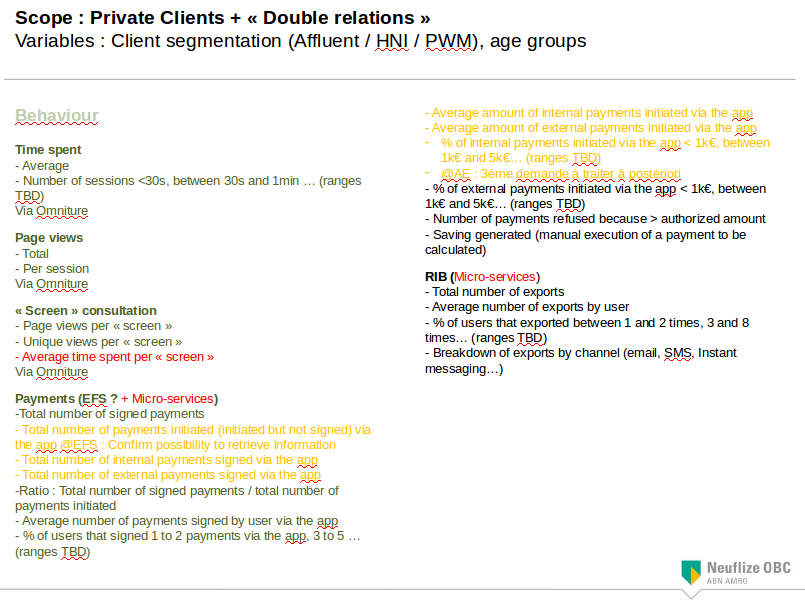
\includegraphics[scale=0.6]{images/travailNeuflizeOBC/dashboard/elkBesoin.png}
	\centering
	\caption{Extrait du besoin client pour le dashboard}
	\label{elkBesoin}
\end{figure}
	
	Une fois cette étude terminée j'ai effectué un rapport auprès d'un architecte du projet qui a validé mon analyse puis j'ai organisé une réunion avec les métiers afin de clarifier la situation et leur faire savoir tout ce qui était faisable par l'API microservices. Au terme de cette réunion et après discussion sur la manière de remplacer certaines informations inaccessibles par d'autres s'en rapprochant ou permettant de les retrouver, j'ai pu me lancer dans la mise en place de la stack ELK et la réalisation du premier jet du dashboard.